\section{Data and Methods}
\label{sec:methods}

\subsection{Workflow overview}
\label{sec:methods_overview}

The workflow is implemented entirely in Google Earth Engine (GEE) and
proceeds in five stages (Figure~\ref{fig:workflow}): (i)~Sentinel-1
acquisition and preprocessing, including an incidence-angle-based orbit
selection; (ii)~automated selection of training samples from global water and
land-cover masks, which removes any manual delineation and makes the workflow
transferable; (iii)~per-acquisition water detection by one of two
\emph{scene-adaptive} classifiers (a single-polarisation Otsu threshold or
a dual-polarisation Support Vector Machine, SVM), both followed by an
\emph{identical} post-processing chain; (iv)~conversion of the cleaned masks
into surface-area time series and per-scene computation of \emph{dynamic}
shoreline morphometry (the area-to-perimeter ratio, A/P, computed from that
scene's own water mask, as distinct from the \emph{static} A/P computed once,
a priori, from the JRC maximum-extent polygon, Section~\ref{sec:methods_ap});
and (v)~validation against reference data
and an audit of computational cost. Keeping every stage identical except the
decision rule is what allows the comparison to isolate the effect of the
classifier itself rather than of the surrounding pipeline.

\begin{figure}[H]
\centering
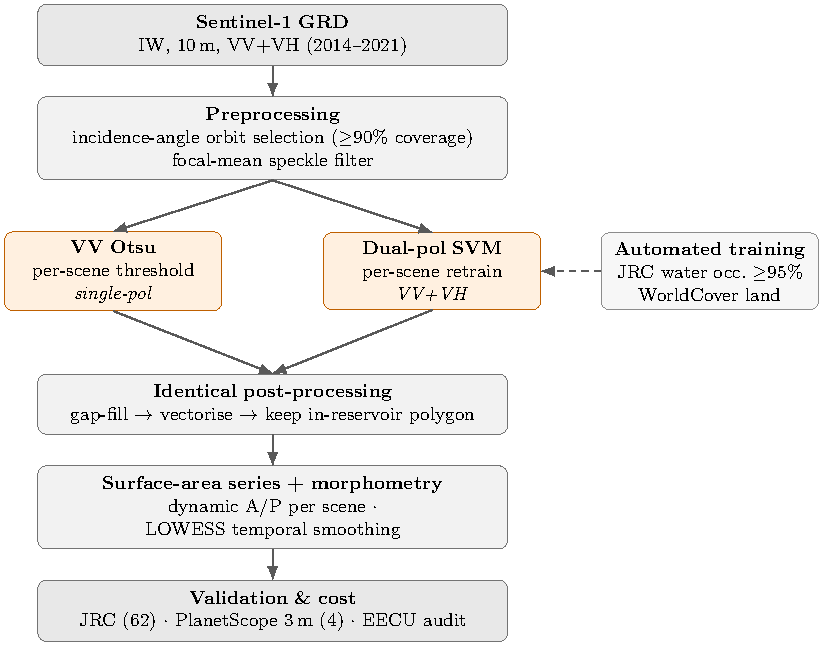
\includegraphics[width=\linewidth]{workflow_diagram.pdf}
\caption{The GEE workflow. A single Sentinel-1 pipeline feeds two
\emph{scene-adaptive} water detectors: a single-polarisation VV Otsu
threshold and a dual-polarisation SVM re-trained per scene (the latter using
training samples drawn automatically from global water and land-cover masks,
dashed). Both masks pass through an \emph{identical} post-processing chain.
Keeping every step common except the decision rule lets the comparison isolate
the classifier. Surface areas and the A/P morphometry feed the validation and
cost audit.}
\label{fig:workflow}
\end{figure}

\subsection{Sentinel-1 data and preprocessing}
\label{sec:methods_s1}

We use the Sentinel-1 C-band Ground Range Detected (GRD) collection in
Interferometric Wide (IW) swath mode at 10~m resolution, with dual
polarisation (VV and VH) \citep{Torres2012}. GEE delivers this product with
thermal-noise removal, radiometric calibration, and terrain correction
already applied. For the global tier, the analysis window spans 1~October~2014 to
31~December~2021, bounded by the availability of the JRC Monthly Water History
used as the reference there (Section~\ref{sec:val_global}). The Sicilian
near-truth tier instead uses acquisitions from May~2024 to May~2025, matching
the availability of the PlanetScope validation imagery
(Section~\ref{sec:val_sicily}). Speckle is
reduced with a 30~m circular focal-mean filter.

Because reservoirs at the edge of the Sentinel-1 swath can be imaged by
several relative orbits with markedly different viewing geometries, we select,
per reservoir, the orbit with the highest mean incidence angle (typically
sub-swath IW3, $\sim$42--46$^{\circ}$) among orbits with at least 20 available
scenes and at least one scene covering $\geq$90\% of the AOI. Within the
chosen orbit, only scenes that reach that same $\geq$90\% coverage are
retained for the time series, falling back to a 50\% threshold only on the
rare orbit where no scene reaches 90\%. An alternative selection rule would
instead maximise scene count or coverage extent, and for swath-edge
reservoirs the two rules can pick different orbits. We prioritise incidence
angle because, in practice, it is the choice that reduces angular
backscatter variability and yields a more temporally consistent series,
which matters more for a per-scene classifier than the raw number of
available scenes. Per-scene coverage gaps within the chosen orbit are filled
by compositing acquisitions within a 6~day window.

\subsection{Automated, transferable training}
\label{sec:methods_training}

To eliminate the manual sample delineation that limits transferability, both
the SVM training samples and the reservoir boundary are derived automatically
from global datasets. The water body itself is the largest polygon of the JRC
maximum-water-extent layer \citep{Pekel2016} within a search radius of the
reservoir location (or of its GRanD/GRDL footprint where a database
identifier is available; \citealp{Lehner2011, Hao2024}). Water training
points are sampled where JRC water \emph{occurrence} is $\geq$95\% (relaxed to
$\geq$80\% where the strict class yields too few points); land training points
are sampled from a 500--2000~m ring around the water body, restricted to
pixels that are non-water in ESA WorldCover \citep{Zanaga2021} and have zero
JRC occurrence. Up to 500 points per class are drawn with a fixed random seed.
Critically, this step fixes only the \emph{locations and labels} of the
samples from multi-decadal, sensor-independent masks; the backscatter values
attached to them are sampled later, which is what enables the scene-adaptive
training below. Figure~\ref{fig:sample_selection} illustrates this automated
selection for one example reservoir, alongside the analogous region used to
build Otsu's per-scene histogram (Section~\ref{sec:methods_otsu}).

\begin{figure}[H]
  \centering
  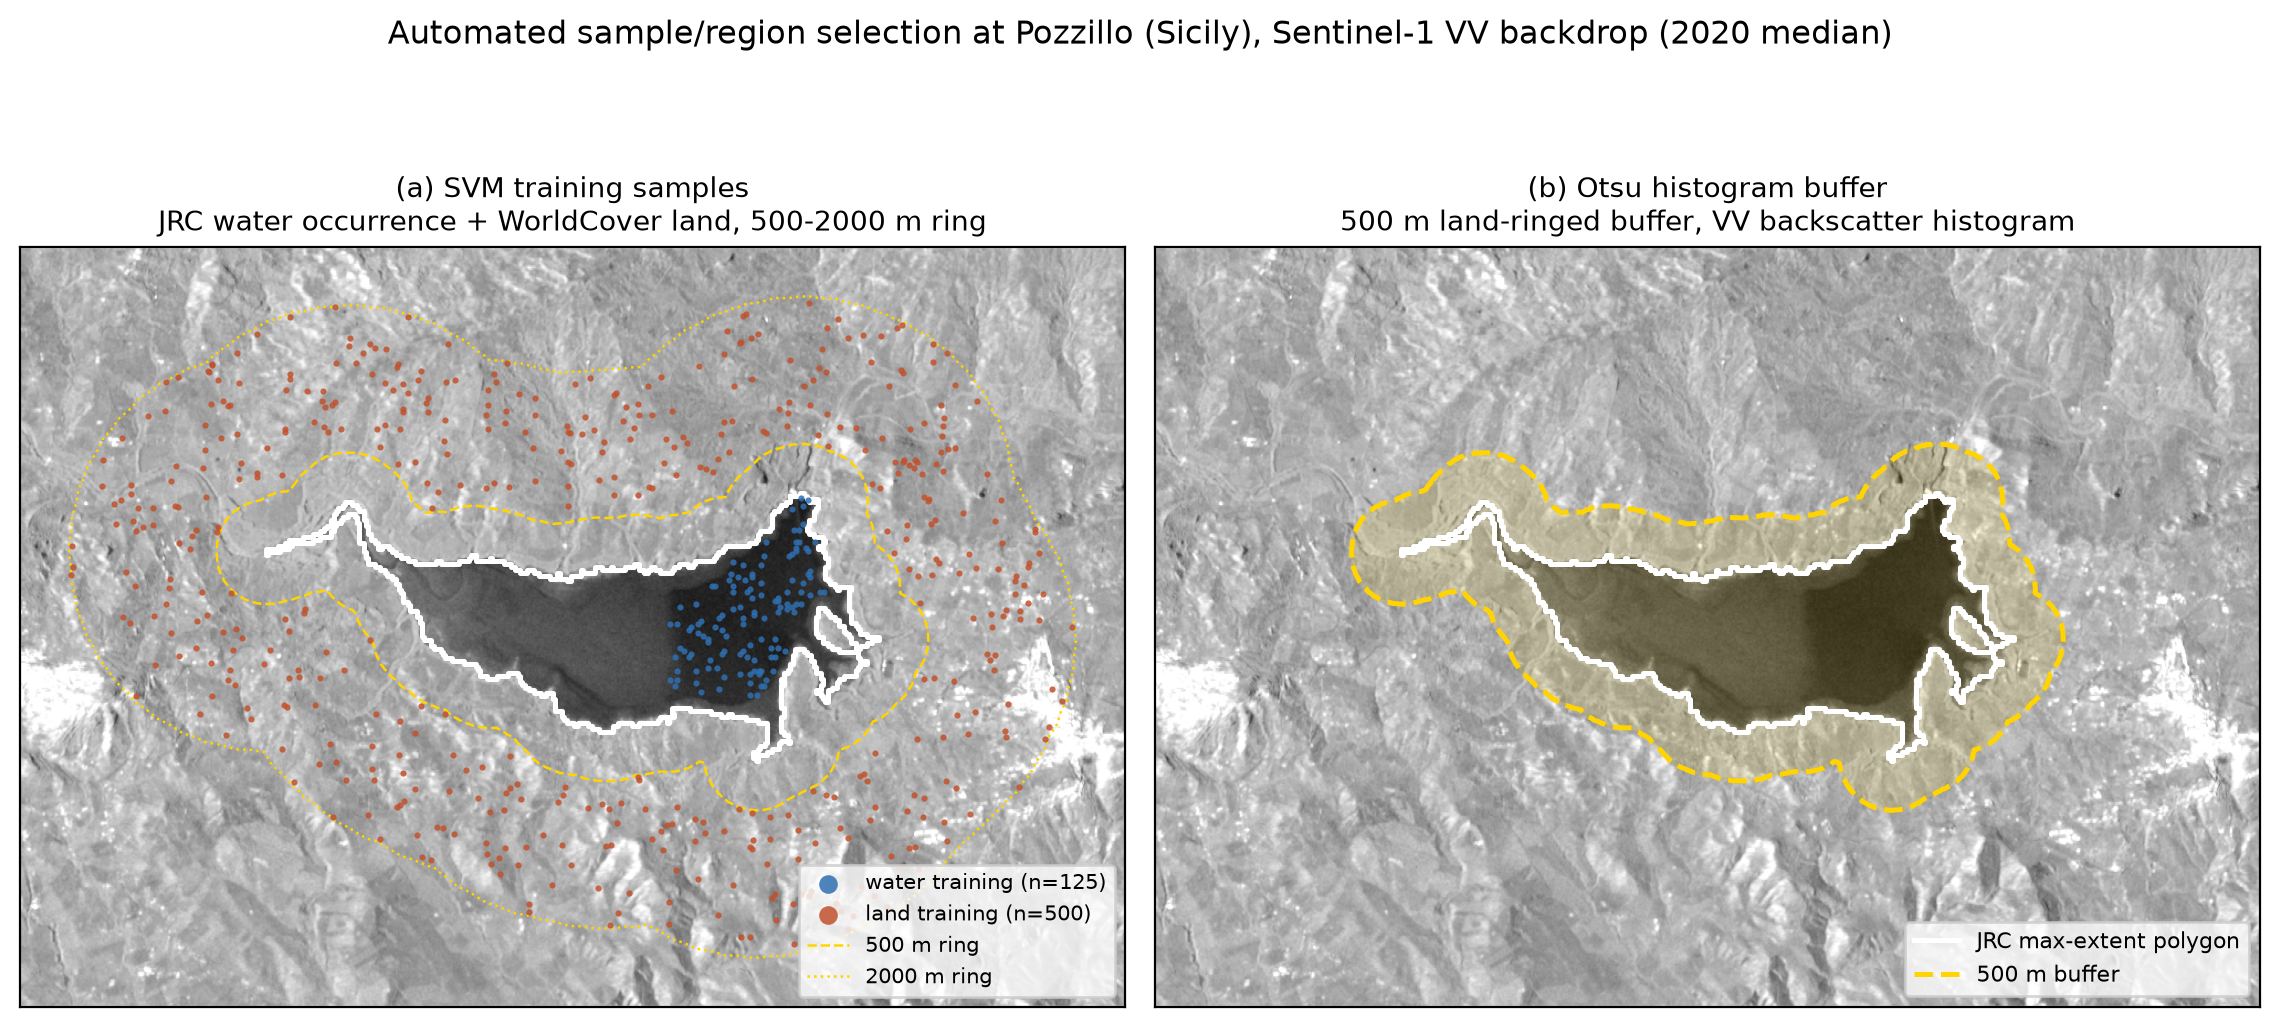
\includegraphics[width=\linewidth]{sample_selection_pozzillo.png}
  \caption{Automated sample and region selection at Pozzillo (Sicily),
  against a Sentinel-1 VV backdrop (2020 median). (a) SVM training points:
  water (JRC occurrence $\geq$95\%) and land (500--2000~m ring, non-water in
  WorldCover, zero JRC occurrence), with the 500~m and 2000~m ring boundaries
  shown for reference. (b) The 500~m land-ringed buffer used to
  build Otsu's per-scene VV backscatter histogram. Both panels share the same
  JRC maximum-extent polygon (white outline).}
  \label{fig:sample_selection}
\end{figure}

\subsection{Two scene-adaptive water detectors}
\label{sec:methods_detectors}

The paper contrasts a single-polarisation threshold with a dual-polarisation
learner, applied under an identical pipeline so that any difference reflects
the \emph{decision rule} (one band vs.\ two) rather than differences in
training regime. Both detectors adapt to each scene's radiometry, which is
essential for a fair comparison: a threshold or boundary fixed once and reused
across all dates cannot absorb the scene-to-scene shifts in backscatter caused
by wind, moisture, and viewing geometry.

\subsubsection{Single-polarisation VV Otsu threshold}
\label{sec:methods_otsu}

For each acquisition, a water threshold is computed on the VV band by Otsu's
between-class-variance maximisation \citep{Otsu1979}: a histogram (256 bins)
of backscatter is built over a 500~m land-ringed buffer around the water
body, which renders it bimodal, and every candidate split of the histogram
into a low- and a high-backscatter class is scored by the variance between
the two resulting class means, weighted by class size. The split that
maximises this between-class variance is the threshold $T_{\text{Otsu}}$,
which is equivalent
to minimising the within-class variance, the criterion Otsu's original 1979
formulation derives a closed-form recursion for. We compute it directly by
evaluating every candidate split over the array-valued histogram (a common
Earth Engine implementation pattern for this exact criterion, rather than
Otsu's original recursive shortcut, which is unnecessary once the histogram
is small enough to score exhaustively), so the criterion being maximised is
unchanged from the 1979 definition. Pixels with $\text{VV} < T_{\text{Otsu}}$
are labelled water, since smooth water has low backscatter. The threshold is
therefore recomputed for every scene and follows the radiometry of that date.

\subsubsection{Dual-polarisation SVM re-trained per scene}
\label{sec:methods_svm}

The dual-polarisation detector is an RBF-kernel SVM
(\texttt{ee.Classifier.libsvm}; \citealp{ChangLin2011}) using VV and VH as
features, with cost $C=1$ and kernel width $\gamma=0.01$. In the scene-adaptive
configuration used for the main comparison, the backscatter of the fixed JRC
training points (Section~\ref{sec:methods_training}) is sampled from
\emph{each scene} and the SVM is re-trained on that scene, producing a
decision boundary that is re-estimated for every acquisition, adapting to
that scene's radiometry the same way Otsu's per-scene threshold does, though
as a nonlinear boundary in the two-band feature space rather than a single
scalar cut. This makes the SVM-vs-Otsu contrast a clean test of the two-band
versus one-band decision rule.

% TODO: once SVM_ADAPTIVE run lands, confirm whether the fixed-2023 SVM variant
% is reported (as an ablation showing the fixed baseline is unfair) or omitted.
A variant that trains the SVM once on a fixed annual (2023) composite is
retained only for the computational-cost audit
(Section~\ref{sec:methods_cost}), where training frequency is irrelevant to the
per-scene inference cost.

\subsection{Post-processing and surface-area time series}
\label{sec:methods_postproc}

Every per-scene water mask is refined by the same sequence: morphological gap
filling via a distance transform, vectorisation of the water pixels, and
retention of the polygon(s) whose centroid falls inside the reservoir boundary
(falling back to the single largest polygon when none qualifies). This
suppresses isolated misclassified patches while preserving disconnected pools
within the reservoir. Surface area is the pixel-area sum of the retained mask
at 10~m. Because water backscatter is sensitive to wind roughness, the
resulting series is temporally filtered with a moving-window outlier removal
followed by LOWESS smoothing \citep{Cleveland1979}, exploiting the
$\sim$6--12~day effective revisit
of the selected orbit. This smoothing is applied outside GEE so that the
accuracy metrics judge the raw classification quality.

\subsection{Shoreline morphometry: the A/P ratio}
\label{sec:methods_ap}

For each reservoir we compute a \emph{static} A/P from the JRC
maximum-extent polygon (area divided by perimeter, in metres). As introduced
in Section~\ref{sec:introduction}, A/P sets
the geometric ceiling on monitorability: for a ground resolution $r$, the
fraction of ambiguous boundary pixels is approximately $r/(A/P)$, so
low-A/P (narrow, dendritic) reservoirs carry proportionally more mixed pixels
and are expected to be harder to delineate regardless of sensor or classifier.
A/P is thus tested as an \emph{a-priori} predictor, computable from
global databases ahead of any image analysis.

For every acquisition, we also compute a \emph{dynamic} A/P from the
perimeter and area of that scene's own retained water mask
(Section~\ref{sec:methods_postproc}), rather than from the JRC polygon.
Because it depends on that day's own classification, dynamic A/P cannot
serve as an a-priori predictor. It is used in
Section~\ref{sec:disc_limitations} to test whether it could instead serve as
a live operational signal for switching between detectors.

\subsection{Validation}
\label{sec:methods_validation}

Skill is measured with the Kling--Gupta Efficiency
\citep[KGE;][]{Gupta2009}, which decomposes into correlation ($r$),
variability ratio ($\alpha$), and bias ratio ($\beta$), reported alongside the
composite score. The comparison between detectors is summarised by
$\Delta\text{KGE} = \text{KGE}_{\text{dual}} - \text{KGE}_{\text{VV}}$ on the
months common to both.

Three further, non-parametric tests support the accuracy comparisons, chosen
because none of the underlying distributions can be assumed normal. Spearman
rank correlation \citep{Spearman1904} is used wherever a monotonic but not
necessarily linear relationship is expected, for example where A/P sets a
ceiling on KGE rather than a linear trend (Section~\ref{sec:res_ap}), since it
does not assume linearity. The Wilcoxon signed-rank test \citep{Wilcoxon1945}
is used for the paired per-reservoir comparison between detectors
(Section~\ref{sec:res_fourway}), since the paired KGE differences are
strongly right-skewed, which would violate the assumption behind a paired
$t$-test. The Kruskal-Wallis test \citep{KruskalWallis1952} compares the KGE
residual across the four climate-zone families (Section~\ref{sec:res_climate}),
appropriate given the small, uneven group sizes ($n=12$--19) where normality
and equal variance cannot be assumed. A worked, hand-checkable example of
each of these four calculations, using small real subsets of the reservoirs
analysed here, is given in the Supplementary Material.

\subsubsection{Global tier: JRC surface-water reference (62 reservoirs)}
\label{sec:val_global}

For the 62 global reservoirs, SAR-derived monthly surface areas are compared
against the JRC Monthly Water History \citep{Pekel2016} (2015--2021), a
globally consistent optical reference at 30~m. This is an inter-product
comparison, not a validation against ground truth, since JRC is itself a
satellite-derived classification product. We therefore apply two
quality-control steps before it enters any result.

\paragraph{De-spiking.} Only months with valid-fraction $\geq$0.90 are
retained; a loose global $3\sigma$ clip removes gross outliers; and an
isolated-excursion filter drops any single month whose value deviates from the
linear interpolation of its neighbours by more than $4\times$ the median
residual (or 12\% of the series median, whichever is larger), gated to apply
only when that month's valid-fraction is below 0.95. This gating matters. It
lets genuine, sustained drawdowns pass, since those occur at near-complete
coverage, while removing isolated optical-contamination spikes, which
coincide with partial coverage.

\paragraph{Reference-noise screening.} De-spiking removes isolated
contamination but not sustained, pervasive reference noise. For every
reservoir we therefore compute a roughness ratio,
$\rho_{\text{rough}} = \operatorname{std}(\Delta\text{JRC}) /
\operatorname{std}(\Delta\text{SAR})$, the month-to-month variability of the
JRC series relative to that of its best-performing SAR detector, on the
months common to both. Genuine hydrological dynamics move both series
together (ratio $\approx$1); a JRC series that jumps while both independent
SAR detectors stay smooth ($\rho_{\text{rough}} \geq 2.5$) indicates the
optical reference itself is unreliable, most often due to cloud, haze, or
riparian-vegetation contamination. Fourteen reservoirs are flagged on this
criterion and excluded from the results that follow, together with four whose
regulated level is nearly constant (a flat reference makes KGE degenerate).
Section~\ref{sec:res_climate}
reports the roughness screen's own diagnostic value: where it does not
resolve a low-agreement case, the residual is attributed to the reference
rather than to the SAR detector.

\subsubsection{Sicilian near-truth: PlanetScope NDWI (4 reservoirs)}
\label{sec:val_sicily}

To break free of JRC's own 30~m mixed-pixel limitation
(Section~\ref{sec:study_sicily}), the four Sicilian reservoirs are
validated against near-truth water masks derived from PlanetScope SuperDove
imagery ($\sim$3~m; \citealp{PlanetTeam2017}) over May~2024--May~2025. Cloud-
free scenes are converted to water masks with a scene-specific NDWI threshold,
produced independently of the SAR workflow. Each PlanetScope observation is
matched one-to-one to the nearest SAR acquisition within $\pm$6~days, and
KGE is computed on the paired series.

% TODO: state final N of PlanetScope scenes / matched pairs per reservoir once
% the SVM_ADAPTIVE Sicily run is downloaded.

\subsection{Computational cost audit}
\label{sec:methods_cost}

Because added complexity is often assumed to raise cost, we test whether
the dual-polarisation classifier is in fact more expensive than the
single-band threshold. We measure Earth Engine Compute Unit (EECU) usage
via \texttt{batchEecuUsageSeconds} (\texttt{ee.data.listOperations}) for
each export task, across four classifier configurations (fixed-training
dual SVM, per-scene VV Otsu, per-scene dual SVM, and a no-post-processing
fast VV variant), pairing tasks per reservoir to compare cost ratios. The
fast configuration isolates the vectorisation lever specifically,
computing area by direct pixel counting rather than the full
vectorisation, keep-polygon, and dynamic-perimeter post-processing chain.

\subsection{Radiometric and climate limits}
\label{sec:methods_wind}

A/P captures a purely \emph{geometric} limit and is blind to
\emph{radiometric} effects, of which we probe two on the reference-noise-screened
62-reservoir set (Section~\ref{sec:val_global}). First, wind: we extract 10~m
wind speed from the hourly ERA5 reanalysis \citep{Hersbach2020} at each
Sentinel-1 overpass (the hourly product is required because overpasses fall near
the diurnal wind extremes) and relate it to the between-method area divergence.
Second, climate: we group reservoirs by K\"oppen--Geiger zone and test, on the
KGE residual after accounting for A/P, whether climate carries a signal beyond
geometry.
